\documentclass[12pt, a4paper]{report}
\usepackage[top=2.5cm, bottom=2.5cm, left=3cm, right=2.5cm]{geometry}
\usepackage{setspace}
\usepackage{titlesec}
\usepackage{graphicx}
\graphicspath{{images/}}
\usepackage{caption}
\usepackage{subcaption}
\usepackage{float}
\usepackage{amsmath}
\usepackage{amssymb}
\usepackage{booktabs}
\usepackage{array}
\usepackage{multirow}
\usepackage{listings}
\usepackage{xcolor}
\usepackage{fancyhdr}
\usepackage{tocloft}
\usepackage[colorlinks=true,linkcolor=black,citecolor=black,urlcolor=blue,
  pdftitle={DC Motor Cascade PI Control System},
  pdfauthor={Yuqi Li}]{hyperref}
\usepackage{appendix}
\usepackage{url}
\usepackage{tikz}
\usepackage{pgfplots}
\pgfplotsset{compat=1.18}

\pagestyle{fancy}
\fancyhf{}
\fancyhead[L]{\small\leftmark}
\fancyhead[R]{\small\thepage}
\fancyfoot{}
\renewcommand{\headrulewidth}{0.4pt}
\onehalfspacing

\titleformat{\chapter}[display]
  {\normalfont\Large\bfseries}{\chaptertitlename~\thechapter}{12pt}{\Large}
\titlespacing*{\chapter}{0pt}{-10pt}{20pt}

\lstdefinestyle{cstyle}{
    language=C,
    basicstyle=\ttfamily\small,
    keywordstyle=\color{blue}\bfseries,
    commentstyle=\color{gray}\itshape,
    stringstyle=\color{orange},
    numbers=left, numberstyle=\tiny\color{gray}, numbersep=8pt,
    frame=single, breaklines=true, tabsize=4,
    showstringspaces=false, captionpos=b,
}
\lstdefinestyle{vhdlstyle}{
    language=VHDL,
    basicstyle=\ttfamily\small,
    keywordstyle=\color{blue}\bfseries,
    commentstyle=\color{gray}\itshape,
    numbers=left, numberstyle=\tiny\color{gray}, numbersep=8pt,
    frame=single, breaklines=true, tabsize=4, captionpos=b,
}

\setcounter{tocdepth}{3}
\setcounter{secnumdepth}{3}

\begin{document}

\begin{titlepage}
  \centering
  \vspace*{2cm}
  {\Large\textbf{Politecnico di Torino}}\\[0.5cm]
  {\large Department of Control and Computer Engineering}\\[2cm]
  \rule{\linewidth}{0.5pt}\\[0.5cm]
  {\LARGE\textbf{DC Motor Cascade PI Control System}}\\[0.3cm]
  {\large Based on STM32F407 and AX309 FPGA}\\[0.5cm]
  \rule{\linewidth}{0.5pt}\\[2cm]
  {\large\begin{tabular}{ll}
    \textbf{Name:}       & Yuqi Li \\[0.3cm]
    \textbf{Student ID:} & s336721 \\[0.3cm]
    \textbf{Course:}     & Electronics for embedded systems \\[0.3cm]
    \textbf{Date:}       & \today \\
  \end{tabular}}
  \vfill
  {\small Academic Year 2025--2026}
\end{titlepage}


\chapter*{Abstract}
\addcontentsline{toc}{chapter}{Abstract}
\markboth{Abstract}{Abstract}

This report presents the design and implementation of a low-speed DC motor control system based on an STM32F407 microcontroller and an AX309 FPGA development board. The system allows the user to set a target speed through a rotary potentiometer. A potentiometer reading below the deadband threshold stops the motor. Above the threshold, the closed-loop running speed is mapped to the range of 15--100 RPM. The STM32 reads the target speed, encoder feedback and motor-current signal, runs a cascade PI control algorithm, and sends a 12-bit duty-cycle command to the FPGA through SPI. The FPGA then generates the PWM signal used by the TB6612FNG motor driver.

The project focuses on register-level implementation. On the MCU side, UART is used for debugging output, ADC for potentiometer and current sampling, TIM3 for quadrature encoder measurement, SPI for Flash and FPGA communication, and I2C for OLED display. The control loop also includes a state machine and startup limits to manage motor start, run and stop transitions. On the FPGA side, the VHDL design includes an SPI slave receiver and a 12-bit PWM generator. The system stores PI parameters in W25Q64 SPI Flash so that tuned parameters can be reloaded after power-on. The final tests verify PWM generation, parameter storage, OLED display, current-sensing functionality and closed-loop speed control.
\\

Keywords: cascade PI, STM32F407, FPGA, DC motor control, register-level programming
\clearpage
\tableofcontents
\clearpage



\chapter{System Design}


\section{Functional Requirements}

This project implements a closed-loop speed control system for a low-speed DC motor. The user sets the desired speed with a rotary potentiometer. When the potentiometer is above the deadband threshold, the microcontroller maps the reading to a running speed in the range of 15--100 RPM. Below the threshold, the motor stops. Encoder feedback provides the measured speed, while the current-sensing circuit provides motor current feedback. Based on these signals, the microcontroller calculates the control output and sends a PWM duty-cycle command to the FPGA through SPI. The FPGA then generates a 12-bit PWM signal for the motor driver.

The system shall provide the following functions:
\begin{itemize}
    \item \textbf{Speed setting and closed-loop control:} support a closed-loop running speed range of 15--100 RPM with a deadband stop zone, and automatically adjust the PWM duty cycle according to encoder and current feedback.
    \item \textbf{Operating status display:} display the motor state, measured speed, PWM duty cycle and motor current on the OLED in real time for direct observation.
    \item \textbf{Debugging output:} speed, current, duty cycle and PI parameters to a PC through UART for runtime monitoring.
    \item \textbf{Non-volatile parameter storage:} store PI parameters in the external W25Q64 SPI Flash. During startup, the microcontroller checks whether valid parameters are available in Flash. If valid data are found, they are loaded.
\end{itemize}
The detailed hardware interfaces, software modules and test results are described in the following chapters.


\section{System Architecture Design}

The overall system architecture is shown in Figure~\ref{fig:architecture}.

\begin{figure}[H]
  \centering
  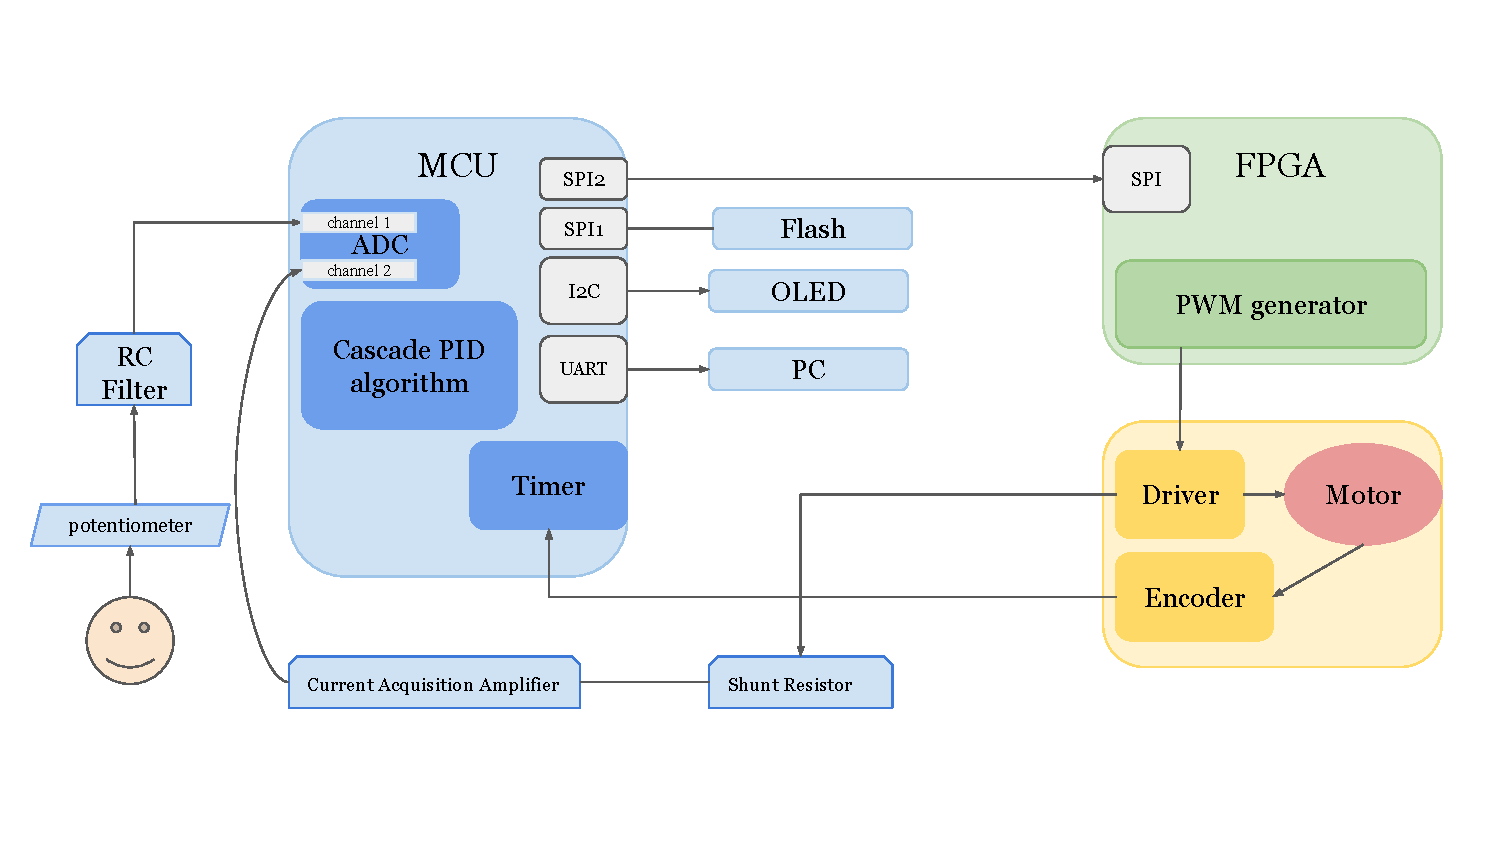
\includegraphics[width=0.95\textwidth]{images/architecture.pdf}
  \caption{System architecture.}
  \label{fig:architecture}
\end{figure}

The system consists of three main parts: the STM32 microcontroller control unit, the FPGA PWM generation unit, and the motor actuation unit. The potentiometer signal is filtered by an RC low-pass circuit, then sampled by the MCU ADC as the target speed. The encoder A/B phases are connected to a timer encoder interface for speed measurement. The current-sensing module measures the motor current in the H-bridge output loop, and its output is sampled by another ADC channel.

The STM32 executes the cascade PI control algorithm using the target speed, measured speed and current. It then sends a duty-cycle command to the FPGA through SPI2. The FPGA generates the PWM waveform, and the H-bridge driver converts this logic signal into the motor drive voltage and current. The Flash memory, OLED and PC are connected to the MCU through SPI1, I2C and UART, respectively, for parameter storage, status display and serial debugging. The main control path is:

\[
\text{Potentiometer} \xrightarrow{\text{RC + ADC}} \text{STM32 PI}
\xrightarrow{\text{SPI2}} \text{FPGA} \xrightarrow{\text{PWM}}
\text{TB6612} \rightarrow \text{Motor}
\]

Encoder speed and current signals are fed back to the STM32 for better control.


\section{Control Strategy}

If only single-loop speed PI is used, the control link can be expressed as:

\[
\text{Target Speed}
\rightarrow \text{Speed PI}
\rightarrow \text{PWM}
\rightarrow \text{Motor}
\]

This structure can regulate speed, but the controller reacts only after the encoder speed has changed. Sometimes, the mechanical response is relatively slow, and the motor current may already increase before the speed feedback shows a clear change. Therefore, this project adds a current loop between the speed loop and the PWM output:

\[
\text{Target Speed}
\rightarrow \text{Speed PI}
\rightarrow \text{Target Current}
\rightarrow \text{Current PI}
\rightarrow \text{PWM}
\rightarrow \text{Motor}
\]

In the cascade PI structure, the speed PI compares the target speed with the encoder speed and outputs a target current. The current PI then compares this target current with the measured motor current and generates the PWM duty cycle. In this way, the speed loop determines how much driving current is needed, while the current loop adjusts the PWM output. The target current is limited so that a large speed error does not directly produce an excessive PWM command.


\chapter{Hardware Implementation}

This chapter explains the specific implementation and connection of each hardware module. The content includes input and feedback links, MCU peripherals and pin distribution, FPGA PWM generator module, motor drive circuit and power supply connection method.


\section{Input and Feedback}


\subsection{Potentiometer and RC Low-pass Filter}

The rotary potentiometer is connected to PA0 as the target speed input. When the potentiometer is turned, its sliding contact may be unstable. The breadboard power supply may also contain switching noise from digital circuits. If the potentiometer is connected directly to the ADC, the sampled value may jump. Therefore, the potentiometer output first passes through an RC low-pass filter before being sent to the ADC. With \(R=10\,\text{k}\Omega\) and \(C=100\,\text{nF}\), the cutoff frequency is
\[
f_c = \frac{1}{2\pi RC} \approx 159\,\text{Hz}.
\]

\begin{figure}[H]
  \centering
  \includegraphics[width=0.6\textwidth]{images/rc_real_board.png}
  \caption{Physical connection of the potentiometer RC filter.}
  \label{fig:breadboard}
\end{figure}

\begin{figure}[H]
  \centering
  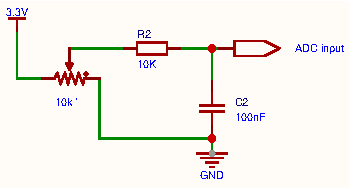
\includegraphics[width=0.85\textwidth]{images/adc_Rc.pdf}
  \caption{Potentiometer input with RC low-pass filter schematic.}
  \label{fig:adc_rc}
\end{figure}

\subsection{Current Sensing}

This project uses an INA240A2 current-sensing module~\cite{ina240} with an R100 shunt resistor. The R100 resistor in the module is connected in series with the motor, and the connection is

\[
\text{AO1} \rightarrow \text{R100} \rightarrow \text{Motor} \rightarrow \text{AO2}.
\]

Therefore, the motor current flows through R100. The IN+ and IN- inputs of the INA240A2 are connected to the two sides of R100 to measure the voltage difference. The shunt resistance is \(0.1\,\Omega\). The INA240A2 amplifies this differential voltage by 50 and sends the output voltage to STM32. By converting this voltage back into current, the system can get the motor current feedback in real time.

\begin{figure}[H]
  \centering
  \includegraphics[width=0.85\textwidth]{images/current_amplifier.pdf}
  \caption{INA240A2 current sensing.}
  \label{fig:ina240}
\end{figure}


The voltage drop on the shunt resistor is proportional to the motor current:
\begin{equation}
V_{\text{shunt}} = I \cdot R_{\text{shunt}}.
\label{eq:shunt_voltage}
\end{equation}

After amplification by the INA240A2, the output voltage is
\begin{equation}
V_{\text{out}} = V_{\text{ref}} + G \cdot V_{\text{shunt}}
= V_{\text{ref}} + G \cdot I \cdot R_{\text{shunt}}.
\label{eq:ina240_out}
\end{equation}
In this module, REF1 is connected to GND and REF2 is connected to VCC. The ideal output voltage when there is no current is:
\begin{equation}
V_{\text{ref}} = \frac{V_{\text{CC}}}{2}.
\end{equation}

In the actual calculation, the measured zero-current voltage \(V_{\text{zero}}\) is used for calibration:
\begin{equation}
I\,[\text{mA}] =
\frac{V_{\text{out}}\,[\text{mV}] - V_{\text{zero}}\,[\text{mV}]}
{50 \times 0.1}
=
\frac{V_{\text{out}} - V_{\text{zero}}}{5}.
\label{eq:current}
\end{equation}

\subsection{Speed Sensing}
The JGA25-370 motor has a Hall-effect quadrature encoder with A and B output signals. The encoder is installed on the internal motor shaft, but the speed to be controlled is the speed of the gearbox output shaft. Therefore, the speed calculation must include both the encoder pulses per revolution and the gear reduction ratio.

In this project, the encoder has 11 PPR, and the gear reduction ratio is 34. TIM3 counts all four edges of the A and B signals, so one revolution of the output shaft gives
\[
11 \times 34 \times 4 = 1496
\]
counts.

If GPIO external interrupts are used, each edge will trigger a CPU interrupt. The interrupt load will also increase when the motor speed becomes higher. In this project, TIM3 is configured in encoder mode. The timer hardware completes the A and B quadrature decoding, and the program only reads the count difference once during each speed update to calculate the speed.

The timer input filter is also enabled to reduce short pulse noise. The speed is calculated as:
\begin{equation}
\text{RPM} =
\frac{\Delta_{\text{count}}}{N_{\text{count}}}
\cdot \frac{60}{T_s}
\label{eq:rpm}
\end{equation}

Here, \(\Delta_{\text{count}}\) is the encoder count change during one speed measurement period. \(T_s\) is the speed update period in seconds. \(N_{\text{count}}\) is the number of encoder counts for one output shaft revolution. It includes the gear reduction ratio and the \(\times 4\) quadrature decoding mode.

In this project, \(N_{\text{count}}=11\times34\times4=1496\). The speed is updated every 10 ms, so \(T_s=0.01\,\text{s}\). One encoder count in this window corresponds to about
\[
\frac{60}{1496\times0.01}\approx4.0\,\text{RPM}.
\]
Therefore, the raw low-speed measurement is quantized. The moving-average filter described later is used to reduce this fluctuation.


\section{Microcontroller}


\subsection{MCU Selection and Specification}
The STM32F407VG is based on an Arm Cortex-M4 core. It can run at up to 168 MHz and has a floating-point unit. Its peripheral resources and processing capability are enough for the 1 kHz interrupt control task in this project. The main peripherals used in this project are shown in Table~\ref{tab:mcu_peripherals}.

\begin{table}[H]
\centering
\caption{STM32F407 peripheral configuration}
\label{tab:mcu_peripherals}
\small
\begin{tabular}{@{}p{0.12\textwidth}p{0.34\textwidth}p{0.44\textwidth}@{}}
\toprule
Peripheral & Function & Configuration \\
\midrule
TIM6 & Control interrupt & TIM6CLK = 84 MHz, update rate = 1 kHz \\
TIM3 & Quadrature encoder interface & TIM3CLK = 84 MHz, speed update period = 10 ms \\
ADC1 & Potentiometer and current sampling & ADC clock = 21 MHz \\
SPI1 & W25Q64 Flash memory & SCK = 5.25 MHz \\
SPI2 & FPGA duty cycle transmission & SCK = 5.25 MHz \\
I2C1 & OLED SSD1306 display & Target SCL = 100 kHz \\
USART2 & Serial debugging through CH340G & 115200 baud \\
\bottomrule
\end{tabular}
\end{table}

\subsection{Pin Allocation and Peripheral Mapping}

Table~\ref{tab:pin_allocation} lists the allocation of all 16 signal pins.
\begin{table}[H]
\centering
\caption{STM32F407 pin allocation}
\label{tab:pin_allocation}
\small
\begin{tabular}{@{}p{0.14\textwidth}p{0.24\textwidth}p{0.52\textwidth}@{}}
\toprule
Pin & Peripheral & Connection Object \\
\midrule
PA0 & ADC1 & Potentiometer (via RC low-pass filter) \\
PA1 & ADC1 & INA240A2 output \\
PA2 & USART2\_TX & CH340G RXD \\
PA3 & USART2\_RX & CH340G TXD \\
PA4 & SPI1\_CS & W25Q64 chip select (software NSS) \\
PA5 & SPI1\_SCK & W25Q64 clock \\
PA6 & SPI1\_MISO & W25Q64 data output (MISO) \\
PA7 & SPI1\_MOSI & W25Q64 data input (MOSI) \\
PB6 & I2C1\_SCL & OLED SCL \\
PB7 & I2C1\_SDA & OLED SDA \\
PB12 & SPI2\_CS & FPGA cs\_n (software NSS) \\
PB13 & SPI2\_SCK & FPGA sck \\
PB14 & SPI2\_MISO & FPGA miso (unused) \\
PB15 & SPI2\_MOSI & FPGA mosi \\
PC6 & TIM3\_CH1 & Encoder phase A \\
PC7 & TIM3\_CH2 & Encoder phase B \\
\bottomrule
\end{tabular}
\end{table}


\section{FPGA PWM Generation}


\subsection{FPGA's Role}
Although the STM32F407 timers can also generate PWM signals, this project uses the FPGA to generate PWM. In this design, the STM32 reads the sensor data, calculates the PI control output, and sends the duty-cycle value through SPI2. Then, the FPGA uses a 50 MHz clock and a 12-bit counter to generate the PWM waveform. This separates PWM generation from the MCU software tasks. The FPGA updates the PWM output after it receives a complete SPI data frame. The key pin connections are shown in Table~\ref{tab:fpga_pins}.

\begin{table}[H]
\centering
\caption{AX309 FPGA pin connections}
\label{tab:fpga_pins}
\small
\begin{tabular}{@{}p{0.20\textwidth}p{0.16\textwidth}p{0.18\textwidth}p{0.36\textwidth}@{}}
\toprule
Signal & FPGA Pin & J3 Header & Connected To \\
\midrule
sck & C15 & J3-21 & STM32 PB13 (SPI2\_SCK) \\
cs\_n & D16 & J3-23 & STM32 PB12 (SPI2\_CS) \\
mosi & C16 & J3-24 & STM32 PB15 (SPI2\_MOSI) \\
miso & E15 & J3-26 & STM32 PB14 (SPI2\_MISO, unused) \\
pwm\_out & F16 & J3-31 & TB6612FNG PWMA \\
\bottomrule
\end{tabular}
\end{table}

\subsection{PWM Frequency}
The AX309 development board has an onboard 50 MHz crystal oscillator. The 12-bit PWM counter overflows after 4096 clock cycles, so the PWM frequency is:

\begin{equation}
f_{\text{PWM}} = \frac{f_{\text{clk}}}{2^{12}} = \frac{50 \times 10^6}{4096}
\approx 12.207\,\text{kHz}
\label{eq:pwm_freq}
\end{equation}

Therefore, the PWM frequency is determined by the FPGA clock frequency and the counter width. At the same time, this counter provides a duty-cycle resolution of about \(100\%/4096 \approx 0.024\%\), which is enough for smooth low-speed adjustment in this project.

\section{Motor Drive Circuit}
The FPGA can only provide a 3.3 V logic signal, so it cannot drive the motor directly. The JGA25-370 motor uses a 12 V supply, and its operating current is much higher than the current that an FPGA I/O pin can provide. Therefore, a TB6612FNG motor driver~\cite{tb6612} is added between the FPGA and the motor. The FPGA outputs the PWM control signal, and the TB6612FNG switches the 12 V motor supply and provides the required drive current.

The PWM signal from the FPGA is connected to the PWMA pin of the TB6612FNG. In this project, AIN1 is connected to 3.3 V, and AIN2 is connected to GND. Therefore, the motor keeps one forward direction, and the system only controls the speed through PWMA. With this direction setting, a high level on PWMA drives the motor in the forward direction, while a low level changes the output to the short-brake state (both outputs pulled low). Therefore, the driver alternates between the drive state and the short-brake state during PWM operation.

For a simplified analysis, the motor terminal voltage can be approximated by the average value:

\[
U_{\text{avg}} \approx D \times 12\,\text{V},
\]

where \(D\) is the PWM duty cycle. The actual current waveform also depends on motor inductance, driver voltage drop, PWM switching behavior and load. The equivalent average voltage for several typical duty cycles is shown in Table~\ref{tab:duty_voltage}.

\begin{table}[H]
\centering
\caption{PWM duty cycle and average voltage}
\label{tab:duty_voltage}
\small
\begin{tabular}{@{}p{0.20\textwidth}p{0.34\textwidth}p{0.36\textwidth}@{}}
\toprule
Duty Cycle & Equivalent Average Voltage & Motor State \\
\midrule
0\% & 0 V & Motor stopped \\
25\% & about 3 V & Low-speed operation \\
50\% & about 6 V & Medium-duty operation \\
100\% & about 12 V & Full-duty operation \\
\bottomrule
\end{tabular}
\end{table}

When the duty cycle increases, the average voltage applied to the motor also increases. As a result, the motor speed usually increases. Therefore, the system controls the motor speed by changing the PWM duty cycle. The TB6612FNG pin connections are shown in Table~\ref{tab:tb6612_wiring}. Figure~\ref{fig:hbridge} shows the basic H-bridge structure. In this figure, VDD is the motor supply, Load is the DC motor, and AO1 and AO2 are the two driver outputs connected to the motor loop.

\begin{figure}[H]
  \centering
  \includegraphics[width=0.55\textwidth]{images/H_principle.png}
  \caption{H-bridge drive principle}
  \label{fig:hbridge}
\end{figure}

\begin{table}[H]
\centering
\caption{TB6612FNG pin connections}
\label{tab:tb6612_wiring}
\small
\begin{tabular}{@{}p{0.18\textwidth}p{0.30\textwidth}p{0.42\textwidth}@{}}
\toprule
TB6612 Pin & Connected To & Notes \\
\midrule
PWMA & FPGA J3-31 (F16) & PWM duty-cycle signal from the FPGA \\
AIN1 & 3.3 V & Direction control: forward rotation \\
AIN2 & GND & Direction control: forward rotation \\
STBY & 3.3 V & Must be pulled high. The chip enters standby mode when this pin is low \\
VCC & 3.3 V & Driver logic supply \\
VM & 12 V supply & Motor drive supply \\
GND & Common ground & Shared with STM32, FPGA, and the current-sensing module \\
AO1 & R100 / INA240A2 IN+ & H-bridge output connected to the motor loop through the shunt resistor \\
AO2 & Motor terminal & Completes the motor output loop \\
\bottomrule
\end{tabular}
\end{table}

\section{Power Supply Design and Noise Suppression}

The system uses separate power supplies for the motor and the logic circuits. At the same time, all modules share a common ground. The STM32F407G-DISC1 and AX309 FPGA development boards are powered by USB from the PC. The TB6612FNG uses two power supplies. VM is connected to the external 12 V DC motor supply, and VCC is connected to the 3.3 V logic supply.

When the motor starts or when the PWM duty cycle changes, the motor current changes. This may cause fluctuation in the supply voltage. Separating the motor supply from the MCU and FPGA logic supplies can reduce the effect of these disturbances on digital communication and ADC sampling. However, a common ground is still needed, so that the PWM, SPI, and ADC signals have the same voltage reference.


\chapter{MCU Register-Level Development}

This chapter explains the implementation of peripherals on the MCU side. USART, ADC, SPI, I2C and timers are initialized and operated mainly through register-level code, while basic functions such as delay use the existing system functions of the project.


\section{Register-Level Peripheral Drivers}
\subsection{UART}

The serial port is used to send the target speed, measured speed, current, duty cycle, and PI intermediate variables to the PC. This makes it easier to observe the system status during debugging. According to the USART configuration requirements in RM0090~\cite{rm0090} and the alternate function table in DS8626~\cite{ds8626}, USART2 is used in this project. Its configuration is shown in Table~\ref{tab:usart2_config}.

\begin{table}[H]
\centering
\caption{USART2 configuration}
\label{tab:usart2_config}
\small
\begin{tabular}{@{}p{0.24\textwidth}p{0.30\textwidth}p{0.36\textwidth}@{}}
\toprule
Requirement & Configuration & Register Setting \\
\midrule
TX and RX & PA2 (TX), PA3 (RX) & GPIOA AF7 \\
Peripheral clock & GPIOA, USART2 & Enable AHB1 and APB1 clocks \\
Baud rate & 115200 baud & Configure BRR \\
Data format & 8N1 & 8 data bits, no parity, 1 stop bit \\
TX/RX enable & Enable TX and RX at the same time & Set TE, RE, and UE to 1 \\
\bottomrule
\end{tabular}
\end{table}

PA2 and PA3 are configured as AF7 alternate function, push-pull output, and no pull-up. According to RM0090~\cite{rm0090}, the reset value of the OVER8 bit in the USART\_CR1 register is 0. This means 16 times oversampling. This project does not change this bit. Therefore, when the APB1 clock is 42 MHz, the baud rate register is calculated as follows:

\[
\text{USARTDIV} = \frac{f_{\text{APB1}}}{16 \times \text{BaudRate}}
= \frac{42{,}000{,}000}{16 \times 115{,}200} \approx 22.786
\quad\Rightarrow\quad \texttt{BRR = 0x16D}
\]

The sending function waits until the TXE flag in the SR register is set. Then it writes data to the DR register. This avoids overwriting bytes that have not been sent yet. USART2 is connected to the PC through an external CH340G USB-to-serial module. PA2 is connected to the RXD pin of the CH340G, PA3 is connected to the TXD pin, and the two boards share a common ground. The serial port parameters are 115200 baud and 8N1.

\subsection{ADC}
The STM32F407 has three ADC peripherals: ADC1, ADC2, and ADC3. This project uses ADC1 to read two analog inputs. PA0 is used to read the potentiometer voltage, and PA1 is used to read the current feedback signal. Each time, the program selects one channel, starts one conversion, waits for the conversion to finish, and then reads the 12-bit result.

The ADC inside the STM32F407 uses a successive approximation register. During sampling, the internal sampling capacitor is connected to the input and stores the input voltage. During conversion, the SAR logic checks the bits from the most significant bit to the least significant bit. The internal DAC generates a test voltage, and the comparator decides whether each bit should be kept or cleared. After 12 comparisons, the final 12-bit result is obtained. The basic structure is shown in Figure~\ref{fig:sar}.

\begin{figure}[H]
  \centering
  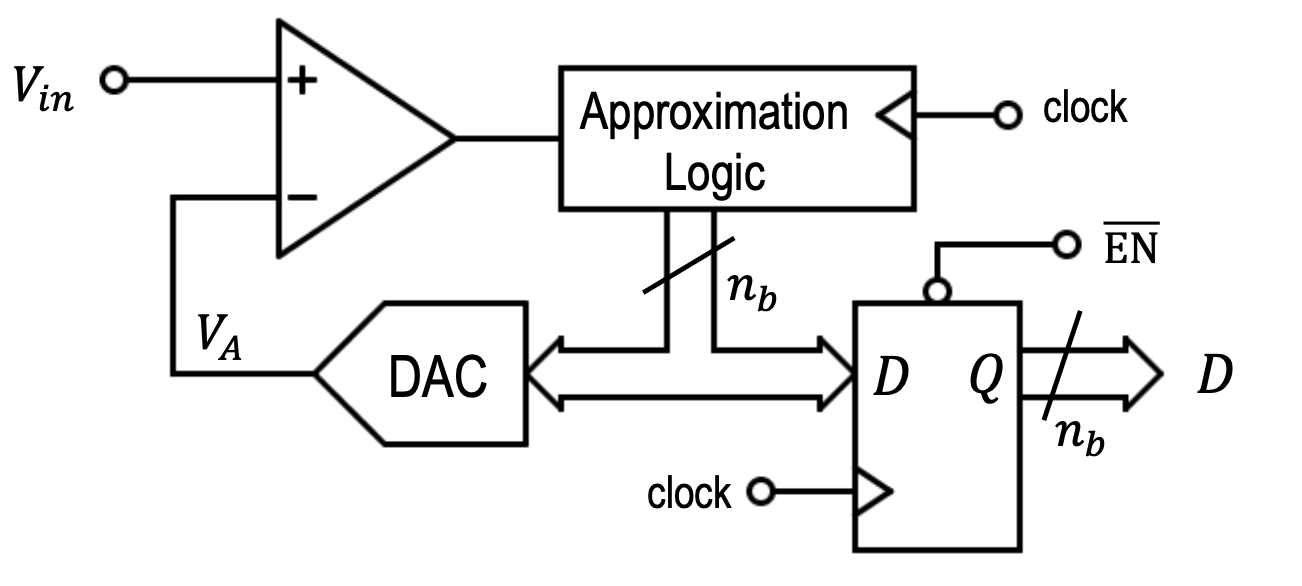
\includegraphics[width=0.85\textwidth]{images/sar.png}
  \caption{SAR ADC structure}
  \label{fig:sar}
\end{figure}

The ADC clock is:

\[
f_{\text{ADCCLK}}=\frac{84\,\text{MHz}}{4}=21\,\text{MHz}.
\]

The corresponding ADC clock period is about \(1/21\,\text{MHz}=47.6\,\text{ns}\). The sampling time is the time when the internal sampling capacitor is connected to the input signal. In general, a higher source impedance needs a longer sampling time, so that the sampling capacitor can be charged more accurately.

The potentiometer output passes through an RC low-pass filter made of a \(10\,\text{k}\Omega\) resistor and a \(100\,\text{nF}\) capacitor. Therefore, a longer sampling time of 144 cycles is used. The current-sense amplifier has a lower output impedance, so a sampling time of 28 cycles is used. The configuration of the two channels is shown in Table~\ref{tab:adc_sampling}.

\begin{table}[H]
\centering
\caption{ADC1 sampling configuration}
\label{tab:adc_sampling}
\small
\begin{tabular}{@{}p{0.25\textwidth}p{0.22\textwidth}p{0.23\textwidth}p{0.20\textwidth}@{}}
\toprule
Sampling Object & Pin & Sampling Time & Use \\
\midrule
Potentiometer output & PA0 & 144 cycles (\(\sim 6.86\,\mu\text{s}\)) & Calculate target speed \\
Current amplifier output & PA1 & 28 cycles (\(\sim 1.33\,\mu\text{s}\)) & Calculate motor current \\
\bottomrule
\end{tabular}
\end{table}

The 12-bit conversion also needs about 12.5 ADC clock cycles. Therefore, the total conversion times of the two channels are about \(7.45\,\mu\text{s}\) and \(1.93\,\mu\text{s}\), respectively.

TIM6 generates an interrupt every 1 ms. In this interrupt, the program reads the potentiometer and current feedback, runs the current loop, and updates the PWM command. The encoder speed and the speed outer loop are updated every 10 ms. The total ADC conversion time is about \(9.38\,\mu\text{s}\), which is less than 1\% of the 1 ms interrupt period. Therefore, the ADC conversion does not significantly affect the other control-loop tasks. The TIM6 configuration is described in the timer section.
\subsection{SPI}

The STM32 communicates with the W25Q64 Flash through SPI1 and sends the 12-bit duty-cycle command to the FPGA through SPI2. The main configuration of the two SPI interfaces is shown in Table~\ref{tab:spi_config}.

\begin{table}[H]
\centering
\caption{SPI configuration}
\label{tab:spi_config}
\small
\begin{tabular}{@{}p{0.15\textwidth}p{0.21\textwidth}p{0.19\textwidth}p{0.17\textwidth}p{0.20\textwidth}@{}}
\toprule
Interface & Device & Clock Frequency & Chip Select & Data Direction \\
\midrule
SPI1 & W25Q64 Flash & 5.25 MHz & PA4 & Bidirectional \\
SPI2 & FPGA & 5.25 MHz & PB12 & Unidirectional (TX only) \\
\bottomrule
\end{tabular}
\end{table}

SPI1 is mounted on the APB2 bus with a clock of 84 MHz. BR[2:0] in SPI1\_CR1 is configured as 011, corresponding to 16 frequency divisions, so

\[
f_{\text{SPI1}}=\frac{84\,\text{MHz}}{16}=5.25\,\text{MHz}.
\]

SPI2 is mounted on the APB1 bus, and the clock is 42 MHz. BR[2:0] in SPI2\_CR1 is configured as 010, corresponding to 8 frequency divisions, so

\[
f_{\text{SPI2}}=\frac{42\,\text{MHz}}{8}=5.25\,\text{MHz}.
\]

The STM32 acts as the master for both SPI peripherals. Both are configured as mode 0 with 8-bit data frames and MSB-first transmission, and the CS signals are controlled by GPIO software.


\subsubsection{SPI1: Flash Memory}

PI parameters stored only in SRAM are lost after power-off. The internal Flash of the STM32 is mainly used for program storage. Therefore, this project uses an external W25Q64 Flash to store PI parameters. After the user saves the parameters, the system can read them again at the next power-on.

The STM32 is the SPI master and generates SCK and CS. MOSI sends data from the STM32 to the Flash, and MISO sends data from the Flash back to the STM32. Pulling CS low selects the Flash, and pulling CS high ends one SPI operation. The W25Q64 does not send data by itself. Each operation is started by the STM32.

The W25Q64FV is an 8 MB SPI NOR Flash memory. It can keep data after power-off. In NOR Flash, programming changes bits from 1 to 0, while erase changes all bits in a sector back to 1. Figure~\ref{fig:flash_prog} shows the basic programming process inside the Flash array.

\begin{figure}[H]
  \centering
  \includegraphics[width=0.40\textwidth]{images/flash1.png}
  \caption{NOR Flash bit programming}
  \label{fig:flash_prog}
\end{figure}

Figure \ref{fig:flash_erase} shows the erase process. During erase, charge is removed from the storage cell, so the bit is restored from 0 to 1.

\begin{figure}[H]
  \centering
  \includegraphics[width=0.40\textwidth]{images/flash2.png}
  \caption{NOR Flash erase process}
  \label{fig:flash_erase}
\end{figure}

Therefore, when updating saved PI parameters, the target sector is erased first and then programmed with new data. The main commands used in this project are shown in Table~\ref{tab:w25q64_cmds}.
\begin{table}[H]
\centering
\caption{W25Q64 instructions}
\label{tab:w25q64_cmds}
\small
\begin{tabular}{@{}p{0.24\textwidth}p{0.20\textwidth}p{0.46\textwidth}@{}}
\toprule
Operation & Command Code & Description \\
\midrule
Read ID & 0x90 & Reads the device ID \\
Write Enable & 0x06 & Enables the next write or erase command \\
Read Data & 0x03 & Reads data from a selected address \\
Page Program & 0x02 & Writes up to 256 bytes \\
Sector Erase & 0x20 & Erases a 4 KB sector to 0xFF \\
Read Status Register & 0x05 & Reads status bits such as BUSY/WIP and WEL \\
\bottomrule
\end{tabular}
\end{table}

Before each write or erase, the STM32 first sends the Write Enable command. This sets the WEL bit in the status register. Without this step, the Flash ignores the write or erase command.

\begin{figure}[H]
  \centering
  \includegraphics[width=0.95\textwidth]{images/flash_page.png}
  \caption{W25Q64 page-program timing}
  \label{fig:flash_page}
\end{figure}

As shown in Figure~\ref{fig:flash_page}, the Page Program command sends 0x02, a 24-bit address and 1--256 bytes of data. When CS goes high, the command ends and the Flash starts writing the data internally. The datasheet~\cite{w25q64} requires CS to stay high for at least 50 ns before the next command. This time is denoted as \(t_{\mathrm{SHSL}}\). During debugging, read operations worked normally but write and erase operations failed because the status register was read too soon after the write or erase command. A 1 ms delay was therefore added before polling the BUSY bit. After this change, write and power-cycle readback worked normally.

The controller parameters are stored at the beginning of Flash sector 0, address 0x000000, and occupy 32 bytes. The stored data include a valid flag, three speed-loop controller parameters, three current-loop controller parameters and a reserved field. The memory layout is shown in Table~\ref{tab:flash_param_layout}. The valid flag uses the fixed value 12345.678f. At startup, the system checks this flag first. If the flag is correct, the six controller parameters are loaded. Otherwise, the default parameters in the program are used.

\begin{table}[H]
\centering
\caption{Flash parameter layout}
\label{tab:flash_param_layout}
\small
\begin{tabular}{@{}p{0.22\textwidth}p{0.20\textwidth}p{0.38\textwidth}@{}}
\toprule
Address Offset & Size & Stored Value \\
\midrule
0x00 & 4 bytes & Valid flag \\
0x04 & 4 bytes & Speed \(K_p\) \\
0x08 & 4 bytes & Speed \(K_i\) \\
0x0C & 4 bytes & Speed \(K_d\) \\
0x10 & 4 bytes & Current \(K_p\) \\
0x14 & 4 bytes & Current \(K_i\) \\
0x18 & 4 bytes & Current \(K_d\) \\
0x1C & 4 bytes & Reserved \\
\bottomrule
\end{tabular}
\end{table}


\subsubsection{SPI2: FPGA}

SPI2 sends the PWM duty-cycle value from the STM32 to the FPGA. One duty-cycle value is sent as two bytes because the PWM command has 12 bits. CS marks the start and end of one transfer. In the current FPGA receiver, the duty value is updated after the second byte is received. The data format is shown in Table~\ref{tab:spi2_frame}.

\begin{table}[H]
\centering
\caption{SPI2 duty frame}
\label{tab:spi2_frame}
\small
\begin{tabular}{@{}p{0.28\textwidth}p{0.22\textwidth}p{0.40\textwidth}@{}}
\toprule
Transfer Order & Bit Field & Content \\
\midrule
Byte 0 & [7:4] & Fixed 0000 \\
Byte 0 & [3:0] & duty[11:8] \\
Byte 1 & [7:0] & duty[7:0] \\
\bottomrule
\end{tabular}
\end{table}

The STM32 splits the 12-bit duty cycle into two bytes. The lower 4 bits of the first byte contain duty[11:8], and the upper 4 bits are filled with zeros. The second byte contains duty[7:0]. The FPGA combines these two bytes into one 12-bit value. SPI2 uses mode 0 and sends the most significant bit first. Its clock is 5.25 MHz, obtained from the APB1 clock divided by 8. Data are only sent from the STM32 to the FPGA, so MISO is not used.


\subsection{I2C}

This project uses I2C1 to drive the SSD1306 OLED~\cite{ssd1306}. The STM32 is the master and generates the clock and data. The OLED is the slave. This project only writes commands and display data to the OLED, so OLED read operation is not used.

I2C does not use a separate CS pin. Instead, the STM32 selects the OLED through the address byte at the beginning of each I2C frame. Both SCL and SDA are open-drain signals. A device can pull the line low or release it, and the pull-up resistor provides the high level. This allows several devices to share the same bus. A START condition begins one transfer, and a STOP condition ends it. After each 8-bit byte, the receiver sends an ACK bit. The main configuration of I2C1 is shown in Table~\ref{tab:i2c_config}.
\begin{table}[H]
\centering
\caption{I2C1 OLED configuration}
\label{tab:i2c_config}
\small
\begin{tabular}{@{}p{0.22\textwidth}p{0.32\textwidth}p{0.36\textwidth}@{}}
\toprule
Item & Configuration & Notes \\
\midrule
Pins & PB6 (SCL), PB7 (SDA) & AF4, open-drain output \\
OLED slave address & 0x3C & 7-bit address \\
Control byte & 0x00 / 0x40 & 0x00 for command, 0x40 for display data \\
APB1 clock & 42 MHz & I2C1 peripheral clock source \\
Target SCL & 100 kHz & Standard mode \\
\bottomrule
\end{tabular}
\end{table}

The SSD1306 slave address is 0x3C in 7-bit form. In an I2C write frame, the peripheral forms the transmitted address byte by shifting this 7-bit address left by one bit and placing the write flag, 0, in the least significant bit:

\[
(\texttt{0x3C} \ll 1) \,|\, 0 = \texttt{0x78}.
\]

After this address byte, the program follows the standard I2C master-write sequence and sends one control byte. A value of 0x00 means that the following bytes are OLED commands, while a value of 0x40 means that the following bytes are display data. Therefore, the OLED write transaction is either a command frame or a data frame:

\[
\text{Command frame: START} \rightarrow \texttt{0x78} \rightarrow \texttt{0x00} \rightarrow \text{command bytes} \rightarrow \text{STOP}.
\]

\[
\text{Data frame: START} \rightarrow \texttt{0x78} \rightarrow \texttt{0x40} \rightarrow \text{display data bytes} \rightarrow \text{STOP}.
\]

\begin{figure}[H]
  \centering
  \includegraphics[width=0.9\textwidth]{images/iic.png}
  \caption{I\textsuperscript{2}C timing}
  \label{fig:i2c_timing}
\end{figure}

I2C1 is located on the APB1 bus, and the input clock is 42 MHz. According to RM0090~\cite{rm0090}, the maximum SCL frequency supported by standard mode is 100 kHz. Therefore,

\[
\texttt{CCR}=\frac{42\,\text{MHz}}{2\times100\,\text{kHz}}=210.
\]

RM0090~\cite{rm0090} also specifies that the maximum SCL rise time in standard mode is 1000 ns. This corresponds to 42 APB1 clock cycles, so TRISE is configured as \(42+1=43\). The final CR2, CCR and TRISE values are 42, 210 and 43. During transmission, bytes are written into \texttt{I2C1->DR} in sequence, and the I2C1 peripheral generates the SCL/SDA timing on PB6 and PB7.


\subsection{Timers}

This project uses TIM3 for encoder counting and TIM6 to trigger the periodic control loop. The configuration is shown in Table~\ref{tab:timer_config}.
\begin{table}[H]
\centering
\caption{Timer configuration}
\label{tab:timer_config}
\small
\begin{tabular}{@{}p{0.18\textwidth}p{0.32\textwidth}p{0.40\textwidth}@{}}
\toprule
Timer & Function & Key Configuration \\
\midrule
TIM3 & Encoder pulse counting & PC6/PC7, encoder mode 3, quadrature \(\times 4\) counting \\
TIM6 & Periodic control interrupt & PSC=83, ARR=999, 1 kHz update interrupt \\
\bottomrule
\end{tabular}
\end{table}

TIM3 counts the rising and falling edges of the two-phase signals of encoder A and B, and enables input digital filtering to suppress short pulse interference. The input clock of TIM6 is 84 MHz. With the prescaler and auto-reload values shown in the table, TIM6 generates an update interrupt every 1 ms. The specific execution process of the control cycle is explained later.


\section{Signal Processing}


\subsection{Moving Average}

The program obtains new samples periodically and averages the most recent \(N\) samples:

\[
\bar{x}[n]=\frac{1}{N}\sum_{k=0}^{N-1}x[n-k].
\]

The longer the window, the smoother the data after filtering, but the slower the response to input changes. This project uses a 16-point sliding average for the slow-changing potentiometer signal and an 8-point sliding average for current and speed signals. Only one new sample is added at each update. The filter does not collect all 16 or 8 samples at once, so the actual time window also depends on the update period of each signal.
\begin{table}[H]
\centering
\caption{Software filter configuration}
\small
\begin{tabular}{@{}p{0.28\textwidth}p{0.20\textwidth}p{0.20\textwidth}p{0.22\textwidth}@{}}
\toprule
Signal & Window Length & Update Period & Time Window \\
\midrule
Potentiometer ADC & 16 samples & 1 ms & 16 ms \\
Encoder RPM & 8 samples & 10 ms & 80 ms \\
Motor current & 8 samples & 1 ms & 8 ms \\
\bottomrule
\end{tabular}
\end{table}


\subsection{Zero-Speed Handling}

During debugging, it was found that the ADC reading was still about 9 even when the potentiometer knob was turned to the minimum position. Although this value is small, direct mapping would still generate a non-zero speed command near the zero position. To avoid unintended motor movement, the program uses a deadband and hysteresis for the potentiometer input.

When the motor is stopped, it only starts if the potentiometer ADC value is greater than or equal to 350. When the motor is running, it only stops if the ADC value is less than or equal to 250. These two thresholds are much higher than the residual zero reading. This gives enough margin for noise and small knob movements near the zero position.

The gap between the start threshold and the stop threshold prevents repeated start-stop switching. After the motor is enabled, the valid speed command is mapped to the range from 15 RPM to 100 RPM:
\[
\text{RPM}_{\text{target}}
=15+\frac{\text{ADC}-350}{4095-350}\times85.
\]

\chapter{Cascade PI Control Algorithm}

This chapter explains the cascade PI control algorithm. The program keeps a general PID calculation function, but \(K_d\) is set to zero in both the speed loop and the current loop. Therefore, this project uses a cascade PI controller. The derivative term is disabled because it can amplify encoder-count fluctuation and current-sampling ripple. This chapter introduces the discrete PI calculation, the cascade structure, the parameter settings and the 1 kHz control loop.


\section{PI Mathematical Model}

The controller calculates its output from the error between the target value and the feedback value. The error is defined as

\[
e(t)=r(t)-y(t),
\]

where \(r(t)\) is the target value, \(y(t)\) is the feedback value, and \(u(t)\) is the controller output. The continuous PID equation is:

\[
u(t) = K_p\,e(t) + K_i\int_0^t e(\tau)\,d\tau + K_d\,\frac{de(t)}{dt}
\]

In this equation, the proportional term responds to the current error, the integral term accumulates past error, and the derivative term responds to error change. In discrete form, the equation used by the program is:

\begin{equation}
u[n] = K_p\,e[n]
+ K_i \sum_{k=0}^{n} e[k]
+ K_d\,\bigl(e[n] - e[n-1]\bigr)
\label{eq:pid_discrete}
\end{equation}

Here, \(e[n]\) is the current error, \(e[n-1]\) is the previous error, and \(u[n]\) is the current controller output. The coefficients \(K_p\), \(K_i\) and \(K_d\) are the discrete gains tuned directly in the program. Because \(K_d=0\) in both loops, the implemented PI equation is

\begin{equation}
u[n] = K_p\,e[n] + K_i \sum_{k=0}^{n} e[k].
\label{eq:pi_discrete}
\end{equation}

If the output has reached its limit while the accumulated error \(\sum e[k]\) continues to increase, the controller may stay saturated for a long time. To reduce this effect, the program limits the accumulated error to the following range:

\[
-I_{\max}
\leq \sum_{k=0}^{n} e[k]
\leq I_{\max}
\]

The controller output is also limited to the range \([u_{\min},u_{\max}]\). The output range of the speed outer loop is 0--400 mA, and the output range of the current inner loop is 0--4095.

In the implementation, the current error is first added to the accumulated error. The controller output is then calculated. If the output exceeds the allowed range and the current error would push it further into saturation, this newly added error is removed. This avoids a large stored error, which would make the controller slow to reduce its output later.
\begin{table}[H]
\centering
\caption{PID/PI symbols}
\small
\begin{tabular}{@{}p{0.22\textwidth}p{0.68\textwidth}@{}}
\toprule
Symbol & Meaning \\
\midrule
\(r\) & target value \\
\(y\) & feedback value \\
\(e=r-y\) & Error between target value and feedback value \\
\(u\) & Control signal generated by the controller \\
\(K_p\) & Effect of the current error on the output \\
\(K_i\) & Effect of the accumulated error on the output \\
\(K_d\) & Effect of the error change on the output \\
\(T\) & Control period of the selected loop \\
\(n\) & Current sample index \\
\(k\) & Summation index in the accumulated-error term \\
\(I_{\max}\) & Absolute upper bound on the accumulated error \\
\(u_{\min}, u_{\max}\) & Lower and upper output limits \\
\bottomrule
\end{tabular}
\end{table}

\section{Cascade Control Structure}

Cascade control uses a speed outer loop and a current inner loop. The speed outer loop calculates the target current from the speed error. A larger target current gives the motor stronger drive. The current inner loop then converts the current error into a 12-bit PWM duty-cycle command. The speed-loop output is limited to 0--400 mA, which also limits the target value of the current inner loop.

\begin{figure}[H]
  \centering
  \resizebox{\textwidth}{!}{%
  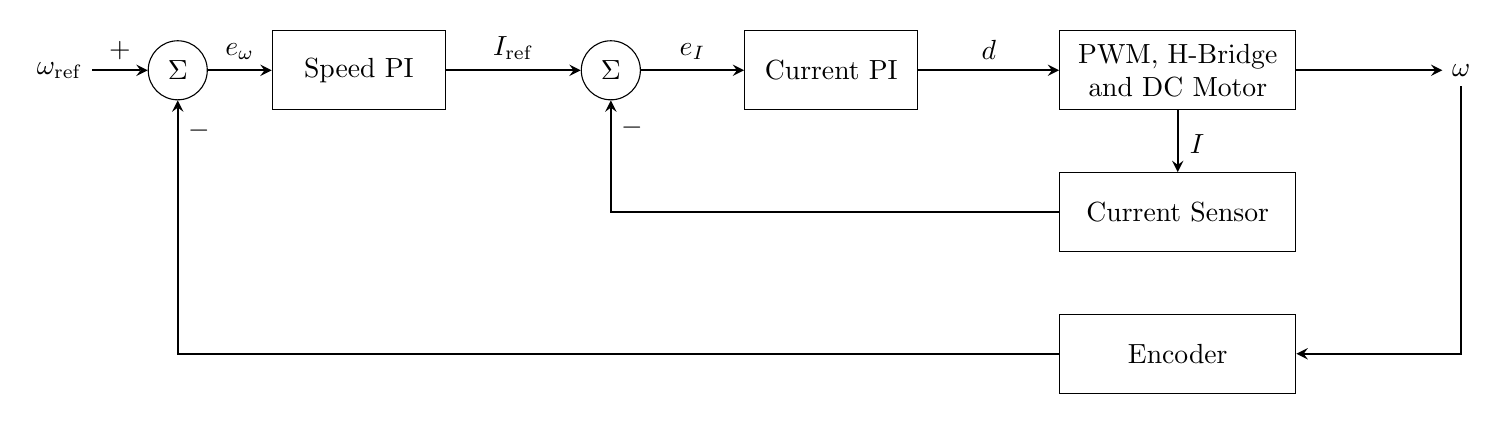
\begin{tikzpicture}[
      >=stealth,
      block/.style={draw, rectangle, minimum width=2.2cm,
                    minimum height=1.0cm, align=center},
      sum/.style={draw, circle, minimum size=0.75cm, inner sep=0pt},
      signal/.style={->, thick}
  ]
      \node (wref) at (0,0) {$\omega_{\mathrm{ref}}$};
      \node[sum] (sumw) at (1.5,0) {$\Sigma$};
      \node[block] (speedpid) at (3.8,0) {Speed PI};
      \node[sum] (sumi) at (7.0,0) {$\Sigma$};
      \node[block] (currentpid) at (9.8,0) {Current PI};
      \node[block, minimum width=3.0cm] (plant) at (14.2,0)
          {PWM, H-Bridge\\and DC Motor};
      \node (wout) at (17.8,0) {$\omega$};

      \node[block, minimum width=3.0cm] (currentfb) at (14.2,-1.8)
          {Current Sensor};
      \node[block, minimum width=3.0cm] (encoder) at (14.2,-3.6)
          {Encoder};

      \draw[signal] (wref) -- node[above] {$+$} (sumw);
      \draw[signal] (sumw) -- node[above] {$e_{\omega}$} (speedpid);
      \draw[signal] (speedpid) -- node[above] {$I_{\mathrm{ref}}$} (sumi);
      \draw[signal] (sumi) -- node[above] {$e_I$} (currentpid);
      \draw[signal] (currentpid) -- node[above] {$d$} (plant);
      \draw[signal] (plant) -- (wout);

      \draw[signal] (plant.south) -- node[pos=0.55, right=3pt, fill=white,
                                           inner sep=1pt] {$I$}
                                    (currentfb.north);
      \draw[signal] (currentfb.west) -| node[pos=0.88, right] {$-$} (sumi.south);

      \draw[signal] (wout.south) |- (encoder.east);
      \draw[signal] (encoder.west) -| node[pos=0.94, right] {$-$} (sumw.south);
  \end{tikzpicture}%
  }
  \caption{Cascade PI block diagram.}
  \label{fig:cascade}
\end{figure}
\begin{table}[H]
\centering
\caption{Cascade PI symbols}
\small
\begin{tabular}{@{}p{0.20\textwidth}p{0.48\textwidth}p{0.22\textwidth}@{}}
\toprule
Symbol & Meaning & Unit / Range \\
\midrule
\(\omega_{\mathrm{ref}}\) & Target speed & RPM \\
\(\omega\) & Measured speed & RPM \\
\(e_{\omega}\) & Speed error: \(\omega_{\mathrm{ref}}-\omega\) & RPM \\
\(I_{\mathrm{ref}}\) & Target current from speed loop & 0--400 mA \\
\(I\) & Measured current from sensing module & mA \\
\(e_I\) & Current error: \(I_{\mathrm{ref}}-I\) & mA \\
\(d\) & PWM duty cycle value sent to FPGA & 0--4095 \\
\bottomrule
\end{tabular}
\end{table}

Cascade control typically requires the inner loop to respond faster than the outer loop~\cite{astrom}. In this project, the current loop runs at 1 kHz, while the speed loop runs every 10 ms, corresponding to 100 Hz. The faster current loop makes the measured current follow the target current before the speed loop updates again. This separates the fast electrical response from the slower mechanical speed response.


\section{PI Parameter Settings}

The two loops use the same PI calculation function, but their gains and output ranges are different. Therefore, their gain values cannot be directly compared. The unit of the speed-loop \(K_p\) is mA/RPM, while the unit of the current-loop \(K_p\) is PWM counts per milliampere.

The speed-loop gains were first tested with larger values. Since the response showed large overshoot, especially during startup, \(K_p\) and \(K_i\) were gradually reduced. The final values were \(K_p=0.8\) and \(K_i=0.01\), as shown in Table~\ref{tab:speed_pi_params}. The no-load steady-state results in Chapter 6 are used to check the final tuning result.
\begin{table}[H]
\centering
\caption{Speed-loop PI parameters}
\label{tab:speed_pi_params}
\small
\begin{tabular}{@{}p{0.20\textwidth}p{0.18\textwidth}p{0.52\textwidth}@{}}
\toprule
Parameter & Value & Notes \\
\midrule
\(K_p\) & 0.8 & Proportional gain \\
\(K_i\) & 0.01 & Integral gain \\
\(u_{\min}\) & 0 mA & Minimum target current \\
\(u_{\max}\) & 400 mA & Maximum target current \\
\(I_{\max}\) & 40000 & Integral limit \\
\bottomrule
\end{tabular}
\end{table}


The current-loop gains were also selected by debugging. The initial values \(K_p=20\) and \(K_i=0.5\) caused clear duty-cycle oscillation because the 1 kHz current loop reacted too strongly to current-error changes. Therefore, the gains were reduced to \(K_p=5.0\) and \(K_i=0.2\), as shown in Table~\ref{tab:current_pi_params}. This reduced the observed duty oscillation during integration.
\begin{table}[H]
\centering
\caption{Current-loop PI parameters}
\label{tab:current_pi_params}
\small
\begin{tabular}{@{}p{0.20\textwidth}p{0.18\textwidth}p{0.52\textwidth}@{}}
\toprule
Parameter & Value & Notes \\
\midrule
\(K_p\) & 5.0 & Proportional gain \\
\(K_i\) & 0.2 & Integral gain \\
\(u_{\min}\) & 0 & Minimum duty cycle \\
\(u_{\max}\) & 4095 & Maximum duty cycle \\
\(I_{\max}\) & 8000 & Integral limit \\
\bottomrule
\end{tabular}
\end{table}


\section{Startup Control}
\subsection{State Machine}

In the early implementation, the program only used a simple motor-enable flag to show whether the motor command was active. The startup stage and the normal running stage used the same control path. In a low-speed startup test, the target speed was about 27.4 RPM, but after the motor started moving, the measured speed reached 66.2 RPM. This happened because static friction kept the motor stopped for a short time. During this time, the speed loop kept accumulating error, so the target current continued to increase.

Therefore, the program introduces a startup state machine in \texttt{motor\_fsm.h}. The state machine does not directly solve the problem by itself. Instead, it separates startup, normal running, and stopping. This allows the program to apply startup-only limits before entering normal closed-loop control.

Similar motor-control projects also use state-based logic to separate different operating stages. For example, ODrive uses calibration states~\cite{odrive_state}, and SimpleFOC uses PWM phase-state handling~\cite{simplefoc_phase_state}. ODrive also discusses velocity-controller windup and integrator-limit handling~\cite{odrive_integrator}.

The state machine contains six states:

\begin{table}[H]
\centering
\caption{Motor state machine}
\label{tab:motor_fsm}
\begin{tabular}{@{}p{0.18\textwidth}p{0.30\textwidth}p{0.42\textwidth}@{}}
\toprule
State & Meaning & Main Action \\
\midrule
\texttt{INIT} & Power-on initial state & Go to \texttt{IDLE} \\
\texttt{IDLE} & Zero-speed region & Keep duty at 0 \\
\texttt{STARTING} & Startup stage & Apply startup limits \\
\texttt{RUNNING} & Normal running & Run cascade PI control \\
\texttt{STOPPING} & Stop command & Reduce duty smoothly \\
\texttt{FAULT} & Reserved fault state & Force duty to 0 \\
\bottomrule
\end{tabular}
\end{table}

Table~\ref{tab:motor_transitions} lists the state transition conditions used during normal operation. Two ADC thresholds are used to form hysteresis. The motor starts when $\text{ADC} \geq 350$ and stops when $\text{ADC} \leq 250$. This prevents repeated start-stop switching near the zero position. The \texttt{FAULT} state is reserved, and there is no trigger for it in the current implementation.

\begin{table}[H]
\centering
\caption{State transition conditions}
\label{tab:motor_transitions}
\begin{tabular}{@{}lll@{}}
\toprule
Current State & Condition & Next State \\
\midrule
\texttt{INIT}     & Initialization complete              & \texttt{IDLE}     \\
\texttt{IDLE}     & $\text{ADC} \geq 350$                & \texttt{STARTING} \\
\texttt{STARTING} & $\text{ADC} \leq 250$                & \texttt{STOPPING} \\
\texttt{STARTING} & $\text{RPM} \geq 12$                 & \texttt{RUNNING}  \\
\texttt{RUNNING}  & $\text{ADC} \leq 250$                & \texttt{STOPPING} \\
\texttt{STOPPING} & $\text{ADC} \geq 350$                & \texttt{STARTING} \\
\texttt{STOPPING} & duty $= 0$ and speed $\approx 0$     & \texttt{IDLE}     \\
\bottomrule
\end{tabular}
\end{table}

In the \texttt{STARTING} state, the target current from the speed loop is limited by a startup current ceiling. The accumulated error in the speed loop is also clamped. When the measured speed reaches 12 RPM, the controller enters the \texttt{RUNNING} state. Before this handoff, the program reduces the stored accumulated error in both the speed loop and the current loop. It also reduces the applied duty cycle. This avoids bringing a large startup command into normal running. Since the minimum normal running command is 15 RPM, the 12 RPM handoff threshold is slightly lower than the minimum speed command for normal running.


\section{Control Loop Implementation}

TIM6 generates an update interrupt every 1 ms. ADC sampling, state-machine update, PI calculation, duty limiting and SPI transmission are completed in this interrupt, so their total execution time must be less than 1 ms. The current inner loop runs every interrupt, while the encoder speed update and speed outer loop run every 10 ms to reduce speed quantization noise. UART and OLED transfers are not performed as blocking display updates inside the 1 kHz interrupt. Instead, the interrupt only stores a telemetry snapshot for later display or serial output. The main execution order is:
\begin{enumerate}
    \item Read the potentiometer and current ADC channels.
    \item Update the encoder speed and speed-loop flag every 10 ms.
    \item Update the motor state machine.
    \item Run the speed loop when due and run the current loop every 1 ms.
    \item Limit the duty command and send the two-byte value to the FPGA through SPI2.
    \item Write one telemetry snapshot for UART and OLED display.
\end{enumerate}

The ADC clock is 21 MHz. The sampling times of the potentiometer and current channels are 144 and 28 ADC clock cycles, respectively, and each 12-bit conversion requires about 12.5 cycles. Therefore, the two-channel conversion time is

\[
t_{\mathrm{ADC}}
=\frac{144+12.5}{21\,\mathrm{MHz}}
+\frac{28+12.5}{21\,\mathrm{MHz}}
\approx 9.38\,\mu\mathrm{s}.
\]

The SPI2 clock is 5.25 MHz. Transmitting two bytes requires 16 SCK cycles:

\[
t_{\mathrm{SPI}}=\frac{16}{5.25\,\mathrm{MHz}}
\approx 3.05\,\mu\mathrm{s}.
\]

The total time of ADC conversion and SPI transmission is about \(12.43\,\mu\text{s}\), which is much shorter than the 1 ms interrupt period. Other operations, such as PI calculation and state-machine update, are simple arithmetic operations, so the 1 ms period has sufficient margin in this implementation.


\chapter{FPGA Development}

The FPGA design contains three VHDL modules. The project is synthesized using Xilinx ISE 14.7, and the target device is the Spartan-6 XC6SLX9-2FTG256.


\section{SPI Slave Receiver}

The SPI slave receiver samples the SPI signals from the STM32 and reconstructs the 12-bit duty-cycle command.


\subsection{SPI Sampling Method}

The final FPGA program uses a simple SPI slave receiver. When CS\_N is low, the receiver uses the external SCK rising edge as the shift clock and samples one MOSI bit on each edge. The \texttt{clk} port is kept for the top-level interface, but this receiver module does not use the FPGA system clock internally. 

\subsection{Two-Byte Duty Cycle Reconstruction}

The PWM duty-cycle value is 12 bits, while SPI2 uses 8-bit data frames. Therefore, the STM32 splits the duty-cycle value into two bytes. The lower 4 bits of the first byte store \(d[11:8]\), and the second byte stores \(d[7:0]\). The reconstruction is

\[
d[11:0]=\{\text{Byte0}[3:0],\,\text{Byte1}[7:0]\}.
\]

After CS\_N is pulled low, the FPGA samples one MOSI bit on each SCK rising edge and records the number of received bits with bit\_cnt. After the first 8-bit byte is received, the lower 4 bits are stored as the high part of the duty-cycle value. After the second byte is received, the two parts are combined into the 12-bit duty\_out signal, and the module generates duty\_valid so that the PWM module can update the duty cycle. The core code is shown below:

\begin{lstlisting}[style=vhdlstyle,caption={SPI duty reconstruction}]
if cs_n = '1' then
 bit_cnt <= 0;
 shift_reg <= (others => '0');
 valid_reg <= '0';

elsif rising_edge(sck) then
 valid_reg <= '0';
 shift_reg <= shift_reg(6 downto 0) & mosi;

 if bit_cnt = 7 then
 temp_hi <= shift_reg(2 downto 0) & mosi;
 bit_cnt <= 8;
 elsif bit_cnt = 15 then
 duty_out <= temp_hi & (shift_reg(6 downto 0) & mosi);
 valid_reg <= '1';
 bit_cnt <= 0;
 else
 bit_cnt <= bit_cnt + 1;
 end if;
end if;
\end{lstlisting}

\section{PWM Generator}

A 12-bit free-running counter is compared with the latched duty-cycle register:
\begin{lstlisting}[style=vhdlstyle,caption={PWM comparator}]
pwm_out <= '1' when counter < duty_latched else '0';
\end{lstlisting}
The PWM logic updates \texttt{duty\_latched} only when \texttt{duty\_valid} is high, and \texttt{duty\_valid} is asserted only after a complete two-byte SPI command is received. This prevents partial-frame data from affecting the PWM output. In the integrated test, the FPGA correctly latched the received 12-bit duty-cycle value and updated the PWM output.

With the comparison \texttt{counter < duty\_latched}, a duty value of 0 keeps the PWM output low at all times. A duty value of 4095 gives \(4095/4096 \approx 99.98\%\), rather than an exact 100\% duty cycle.


\section{Top-Level Integration}

\texttt{top.vhd} connects the SPI receiver and the PWM generator. The SPI receiver outputs the 12-bit duty-cycle value and a data-valid signal. When the PWM module receives the valid signal, it updates the duty-cycle register and generates the PWM output. The FPGA pins for each input and output signal are specified in \texttt{pin.ucf}. The corresponding physical connections are listed in Table~\ref{tab:fpga_pins}.
\chapter{Testing}

This chapter presents the test results after the STM32F407, FPGA, motor driver, encoder, and current-sensing circuit were connected. The tests include PWM duty-cycle transmission, parameter storage, OLED display, current sensing, no-load steady-state speed accuracy, startup behavior, and a simple manual disturbance test.


\section{Experimental Results}
The system sends one telemetry line over UART every 200 ms. Each line uses the following format:

\begin{center}
\texttt{[STATE] set=X RPM=X duty=X adc=X curr\_raw=X iset=XmA curr=XmA}
\end{center}

Table~\ref{tab:uart_fields} explains the meaning of each field.

\begin{table}[H]
\centering
\caption{UART telemetry fields}
\label{tab:uart_fields}
\small
\begin{tabular}{@{}p{0.14\textwidth}p{0.18\textwidth}p{0.58\textwidth}@{}}
\toprule
Field & Unit & Description \\
\midrule
\texttt{[STATE]} & --- & Motor state: \texttt{IDLE}, \texttt{START}, \texttt{RUN}, or \texttt{STOP}. \\
\texttt{set} & RPM & Target speed from the potentiometer ADC value. \\
\texttt{setR} & RPM & Ramp-limited speed setpoint used to reduce overshoot from sudden potentiometer changes. This field was later removed because the \texttt{START} state already limits startup current. \\
\texttt{RPM} & RPM & Measured motor speed from the TIM3 encoder count over 10 ms. \\
\texttt{duty} & counts & 12-bit PWM duty-cycle command sent to the FPGA, from 0 to 4095. \\
\texttt{adc} & counts & Raw potentiometer ADC reading before speed mapping. \\
\texttt{curr\_raw} & counts & Raw current-sensor ADC reading before offset removal and gain conversion. \\
\texttt{iset} & mA & Current setpoint from the speed loop. \\
\texttt{curr} & mA & Measured motor current after offset calibration and INA240A2 gain conversion. \\
\bottomrule
\end{tabular}
\end{table}

\subsection{System Operation Status}

After power-on, the OLED shows the motor state, measured speed, PWM duty cycle, and motor current. The main system variables can be observed.

\begin{figure}[H]
\centering
\includegraphics[width=0.80\textwidth]{\detokenize{images/oled_real.png}}
\caption{OLED display showing motor state, speed, duty cycle, and current.}
\label{fig:system_oled}
\end{figure}

\subsection{FPGA PWM Output}
The FPGA uses a 50 MHz clock and a 12-bit counter to generate the PWM signal. Therefore, the theoretical PWM frequency is
\[
f_{\mathrm{PWM}}=
\frac{50\,\mathrm{MHz}}{4096}
=12.20703125\,\mathrm{kHz}.
\]

In the integrated test, the STM32 sent a 12-bit duty-cycle command to the FPGA through SPI2. After receiving the command, the FPGA updated the PWM output. The motor speed changed according to the duty-cycle command from the control loop. The test verifies the basic SPI duty-cycle transmission and the FPGA PWM driving path.
\begin{figure}[H]
\centering
\includegraphics[width=0.85\textwidth]{\detokenize{images/pwm_la2016.png}}
\caption{FPGA PWM output waveform captured by a logic analyser.}
\label{fig:pwm_wave}
\end{figure}

\subsection{W25Q64 Parameter Storage}

The device ID read from the W25Q64 Flash was 0xEF16. After the PI parameters were changed and saved through the serial interface, the same values could still be loaded after power on. This shows that parameter saving and power-on loading worked correctly.

\begin{figure}[H]
\centering
\includegraphics[width=0.8\textwidth]{\detokenize{images/flash_serial.png}}
\caption{UART log showing the saved PI parameters loaded after power-on.}
\label{fig:flash_cycle}
\end{figure}

\subsection{Current Sensing}
When the motor current was zero, the raw current-sensing ADC value, shown as \texttt{curr\_raw} in the UART log, was about 2038. With a 3.3 V ADC reference voltage, this value corresponds to an INA240A2 output voltage of about 1.642 V. The software used this measured zero-current value as the calibration offset.

In the no-load steady-state tests, the calculated motor current was usually about 40--55 mA during stable operation. The UART log in Fig. 6.4 shows several examples where \texttt{curr\_raw} changed with the motor operating state.


\begin{figure}[H]
\centering
\includegraphics[width=0.85\textwidth]{\detokenize{images/current_sensing.png}}
\caption{UART log of current ADC samples and motor current.}
\label{fig:current_meas}
\end{figure}

\subsection{Steady RPM Error}
Four no-load operating points were tested. The results are shown in Table~\ref{tab:steady_accuracy}.

\begin{table}[H]
\centering
\caption{Steady-state speed accuracy}
\label{tab:steady_accuracy}
\small
\begin{tabular}{@{}lccccc@{}}
\toprule
Nominal Speed & Setpoint & Mean RPM & RPM Range & Error & Overshoot \\
\midrule
20 RPM  & 21.4  & 21.5 & 20.6--22.1   & -0.5\% & about 5\% \\
50 RPM  & 50.5  & 50.2 & 49.6--50.6   & +0.6\% & 4.2\% \\
80 RPM  & 80.8  & 80.3 & 79.7--80.7   & +0.6\% & about 0\% \\
100 RPM & 100.0 & 99.9 & 99.3--100.3 & +0.1\% & about 0\% \\
\bottomrule
\end{tabular}
\end{table}

The error is calculated as
\[
\mathrm{Error}=
\frac{\mathrm{Setpoint}-\mathrm{Mean\ RPM}}
{\mathrm{Setpoint}}
\times 100\%.
\]

The steady-state error of all four test points was less than 1\%. The remaining speed fluctuation was mainly caused by encoder speed quantisation in the sampling window. The observed fluctuation range was about $(\pm 0.5)$--$(\pm 0.75)$\,RPM.




\subsection{Startup and Disturbance Tests}

\begin{figure}[H]
\centering
\includegraphics[width=0.85\textwidth]{\detokenize{images/lowspeed_final.png}}
\caption{Low-speed startup: speed and current.}
\label{fig:lowspeed_startup}
\end{figure}
In the low-speed startup test, the controller changed from \texttt{IDLE} to \texttt{START}. While the motor was still stopped, the controller gradually increased the target current. After the motor started to rotate, the system entered the \texttt{RUN} state. Finally, the speed stayed close to the target value of 26.7 RPM. 

\begin{figure}[H]
\centering
\includegraphics[width=0.85\textwidth]{\detokenize{images/highspeed_final.png}}
\caption{High-speed startup: speed and current.}
\label{fig:highspeed_startup}
\end{figure}
During the disturbance, the added friction increased the motor load and caused the speed to drop below the 20.2 RPM reference. The speed loop then increased the current setpoint \texttt{iset} from about 50--51 mA to about 58 mA, allowing the motor to produce more torque against the disturbance.

When the disturbance was released, the load suddenly decreased, but \texttt{iset} did not immediately return to its original value because of the integral action. As a result, the motor speed briefly rose above the reference, reaching about 25--28 RPM. After that, the speed loop reduced \texttt{iset}, and the speed returned to around 20 RPM. This shows the basic disturbance response of the cascade speed-current control structure.
\begin{figure}[H]
\centering
\includegraphics[width=0.85\textwidth]{\detokenize{images/manual.png}}
\caption{Speed and current response during the manual disturbance test at 20 RPM.}
\label{fig:disturbance}
\end{figure}


\chapter{Conclusion}

This project implements a low-speed DC motor control system based on an STM32F407 and an AX309 FPGA board. The STM32 reads the potentiometer, encoder, and motor-current signals. It runs the cascade PI controller, stores the tuned PI parameters in W25Q64 Flash, and sends a 12-bit duty-cycle command to the FPGA through SPI. The FPGA receives the duty-cycle command and generates the PWM signal for the TB6612FNG motor driver.

The final system verifies the main functional path, including OLED status display, Flash parameter saving and loading, current sensing, FPGA PWM output, and disturbance test. At the tested operating points, the steady-state speed error was less than 1\%.


\begin{thebibliography}{9}

\bibitem{rm0090}
  STMicroelectronics, \textit{RM0090 Reference Manual: STM32F405/415/407/417/427/437/429/439 Arm-based 32-bit MCUs}, Rev.~19, 2021.
  [Online]. Available: \url{https://www.st.com}. Accessed: Jun. 22, 2026.

\bibitem{ds8626}
  STMicroelectronics, \textit{DS8626 Datasheet: STM32F407xx}, 2020.
  [Online]. Available: \url{https://www.st.com}. Accessed: Jun. 22, 2026.

\bibitem{ina240}
  Texas Instruments, \textit{INA240 Bidirectional, Zero-Drift, High/Low-Side Current-Sense Amplifier}, SBOS566D, 2015.
  [Online]. Available: \url{https://www.ti.com}. Accessed: Jun. 22, 2026.

\bibitem{w25q64}
  Winbond Electronics, \textit{W25Q64FV 64M-Bit Serial Flash Memory}, 2015.
  [Online]. Available: \url{https://www.winbond.com}. Accessed: Jun. 22, 2026.

\bibitem{tb6612}
  Toshiba, \textit{TB6612FNG Dual DC Motor Driver IC Datasheet}, 2008.
  [Online]. Available: \url{https://toshiba.semicon-storage.com}. Accessed: Jun. 22, 2026.

\bibitem{ssd1306}
  Solomon Systech, \textit{SSD1306 128$\times$64 OLED Controller Datasheet}, 2008.
  [Online]. Available: \url{https://www.solomon-systech.com}. Accessed: Jun. 22, 2026.

\bibitem{astrom}
  K.~J.\ {\AA}str\"om and T.\ H\"agglund,
  \textit{Advanced PID Control}.
  ISA, 2006.

\bibitem{odrive_integrator}
  ODrive Robotics, ``Added integrator\_limit to allow prevention of integrator windup,''
  Pull Request \#626, 2021.
  [Online]. Available: \url{https://github.com/odriverobotics/ODrive/pull/626}. Accessed: Jun. 22, 2026.

\bibitem{odrive_state}
  ODrive Robotics, ``Make encoder index search and encoder offset calibration independent,''
  Commit 69e1b533, 2018.
  [Online]. Available: \url{https://github.com/odriverobotics/ODrive/commit/69e1b5331a059ebdf8a5375c3843ddc456d1728e}. Accessed: Jun. 22, 2026.

\bibitem{simplefoc_phase_state}
  SimpleFOC, ``Update teensy4\_mcu.cpp \_writeDutyCycle6PWM to handle phase\_state,''
  Commit a916bfaa, 2025.
  [Online]. Available: \url{https://github.com/simplefoc/Arduino-FOC/commit/a916bfaa015085da923ac1164098c0593b5eb381}. Accessed: Jun. 22, 2026.

\end{thebibliography}

\appendix

\chapter{Key Source Code}


\section{Pseudo-code of the 1\,kHz PI Control Loop}


\begin{lstlisting}[style=cstyle,caption={Pseudo-code of the 1 kHz control loop}]
void TIM6_DAC_IRQHandler(void)
{
 if (TIM6 update flag is set) {
  clear TIM6 update flag;

  read potentiometer ADC and current ADC;
  update filtered current feedback;

  if (10 ms elapsed) {
   update TIM3 encoder speed;
   enable one speed-loop update;
  }

  update motor state machine;

  if (state is STARTING or RUNNING) {
   if (speed-loop update is due) {
    apply minimum run command;
    calculate target current with speed PI;
    apply startup current and integral limits when needed;
   }

   calculate duty command with current PI;
   apply duty slew and duty limits;
  } else {
   reset PI output or decrease duty during stopping;
  }

  send the 12-bit duty value to the FPGA through SPI2;
  save one telemetry snapshot for UART and OLED display;
 }
}
\end{lstlisting}

\section{Positional-Form PID Implementation}


\begin{lstlisting}[style=cstyle,caption={PID calculation function, with kd set to zero for PI control}]
float PID_Calc(PID_TypeDef *pid, float setpoint, float feedback)
{
 float err = setpoint - feedback;

 pid->integral += err;
 if (pid->integral > pid->integral_max)
 pid->integral = pid->integral_max;
 else if (pid->integral < -pid->integral_max)
 pid->integral = -pid->integral_max;

 float deriv = pid->kd * (err - pid->err_prev);
 pid->err_prev = err;

 float output = pid->kp * err + pid->ki * pid->integral + deriv;

 if (output > pid->out_max) {
 output = pid->out_max;
 if (err > 0.0f) pid->integral -= err;
 } else if (output < pid->out_min) {
 output = pid->out_min;
 if (err < 0.0f) pid->integral -= err;
 }
 return output;
}
\end{lstlisting}
\end{document}
